% !TeX program = xelatex
\documentclass[a4paper,10pt]{article}

% ============================================================================
% ១. កញ្ចប់បណ្ណាល័យ និងការកំណត់ទំព័រ (Packages & Page Setup — តាមគំរូ ls_plan.tex)
% ============================================================================
\usepackage[a4paper, left=0.95cm, right=0.95cm, top=0.85cm, bottom=0.92cm, footskip=0.52cm]{geometry}
\usepackage{amsmath}
\usepackage{unicode-math}
\usepackage{fontspec}
\usepackage{longtable, array, multirow, colortbl}
\usepackage[table]{xcolor}
\usepackage{enumitem}
\usepackage{pifont}
\usepackage{fancyhdr}
\usepackage{tikz}
\usetikzlibrary{calc, arrows.meta, decorations.pathreplacing, patterns, positioning, babel}

\makeatletter
\let\@expl@@@mark@update@singlecol@structures@@\relax
\makeatother

% --- ប្រព័ន្ធស្វែងរកទីតាំងពុម្ពអក្សរស្វ័យប្រវត្តិ (Windows Local + Cloud Repo fonts/) ---
\providecommand{\NGSFindFonts}{%
  \IfFileExists{C:/Windows/Fonts/cambria.ttc}{%
    \def\NGSSysPath{C:/Windows/Fonts/}%
    \def\NGSUserPath{C:/Users/KIT/AppData/Local/Microsoft/Windows/Fonts/}%
  }{%
    \IfFileExists{./fonts/KhmerOSsiemreap.ttf}{\def\NGSSysPath{./fonts/}\def\NGSUserPath{./fonts/}}{%
    \IfFileExists{../fonts/KhmerOSsiemreap.ttf}{\def\NGSSysPath{../fonts/}\def\NGSUserPath{../fonts/}}{%
    \IfFileExists{../../fonts/KhmerOSsiemreap.ttf}{\def\NGSSysPath{../../fonts/}\def\NGSUserPath{../../fonts/}}{%
    \IfFileExists{../../../fonts/KhmerOSsiemreap.ttf}{\def\NGSSysPath{../../../fonts/}\def\NGSUserPath{../../../fonts/}}{%
    \IfFileExists{../../../../fonts/KhmerOSsiemreap.ttf}{\def\NGSSysPath{../../../../fonts/}\def\NGSUserPath{../../../../fonts/}}{%
    \IfFileExists{../../../../../fonts/KhmerOSsiemreap.ttf}{\def\NGSSysPath{../../../../../fonts/}\def\NGSUserPath{../../../../../fonts/}}{%
    \IfFileExists{../../../../../../fonts/KhmerOSsiemreap.ttf}{\def\NGSSysPath{../../../../../../fonts/}\def\NGSUserPath{../../../../../../fonts/}}{%
      \def\NGSSysPath{../../../../../../../fonts/}\def\NGSUserPath{../../../../../../../fonts/}%
    }}}}}}}%
  }%
}
\NGSFindFonts

% ============================================================================
% ២. កំណត់ពុម្ពអក្សរ (Fonts — តាមគំរូ ls_plan.tex)
% ============================================================================
\setmathfont[Path={\NGSSysPath}, FontIndex=1, Scale=1.02]{cambria.ttc}
\defaultfontfeatures{Ligatures=TeX}

\setmainfont[
  Path={\NGSUserPath},
  Extension=.ttf,
  Script=Khmer,
  BoldFont={KhmerOSsiemreap},
  BoldFeatures={FakeBold=1.8},
  ItalicFont={KhmerOSsiemreap},
  ItalicFeatures={FakeSlant=0.25},
  BoldItalicFont={KhmerOSsiemreap},
  BoldItalicFeatures={FakeBold=1.8, FakeSlant=0.25}
]{KhmerOSsiemreap}

\newfontfamily\muol[Path={\NGSUserPath}, Extension=.ttf, Script=Khmer]{KhmerOSmuollight}
\newfontfamily\Tacteing[Path={\NGSUserPath}, Extension=.TTF]{TACTENG}
\newfontfamily\TimesEn[Path={\NGSSysPath}, Extension=.ttf, BoldFont={timesbd}, ItalicFont={timesi}, BoldItalicFont={timesbi}]{times}
\newfontfamily\CalibriFont[Path={\NGSSysPath}, Extension=.ttf]{calibri}
\newfontfamily\CourierCirc[Path={\NGSSysPath}, Extension=.ttf]{cour}

\XeTeXlinebreaklocale "km"
\XeTeXlinebreakskip = 0pt plus 1pt minus 0.1pt

% ============================================================================
% ៣. ពណ៌ និងការតុបតែង (Colors & Styles)
% ============================================================================
\definecolor{stepbg}{HTML}{D9D9D9}
\definecolor{headgray}{HTML}{E6E6E6}
\definecolor{emphred}{HTML}{C00000}

\pagestyle{fancy}
\fancyhf{}
\renewcommand{\headrulewidth}{0pt}
\fancyfoot[R]{\CalibriFont\fontsize{9pt}{11pt}\selectfont\thepage}

\setlength{\parindent}{0pt}
\setlength{\parskip}{0pt}
\setlength{\tabcolsep}{4.5pt}
\setlength{\LTpre}{2pt}
\setlength{\LTpost}{2pt}

\newcolumntype{L}[1]{>{\raggedright\arraybackslash}p{#1}}
\newcolumntype{C}[1]{>{\centering\arraybackslash}p{#1}}

% ============================================================================
% ៤. ពាក្យបញ្ជាជំនួយ (Helper Macros)
% ============================================================================
\newcommand{\en}[1]{{\TimesEn #1}}
\newcommand{\enbf}[1]{{\TimesEn\bfseries #1}}
\newcommand{\khmflourish}{{\Tacteing\fontsize{15pt}{15pt}\selectfont 3}}
\newcommand{\wcirc}{{\CourierCirc\fontsize{9.5pt}{11pt}\selectfont o}}
\newcommand{\ditem}{{\fontsize{7.5pt}{10pt}\selectfont\ding{117}}\ }
\newcommand{\fiveE}[1]{\textcolor{emphred}{\CalibriFont\bfseries #1}}
\newcommand{\redsub}[1]{\textcolor{emphred}{#1}}
\newcommand{\timenote}[1]{\textcolor{emphred}{\textit{#1}}}
\newcommand{\stepheader}[1]{\multicolumn{3}{|c|}{\cellcolor{stepbg}\muol #1} \\ \hline}
\newcommand{\cfig}[1]{{\centering\vspace{3pt}#1\vspace{3pt}\par}}
\newcommand{\cnum}[1]{\mbox{\fontsize{10.5pt}{12pt}\selectfont\ding{\numexpr181+#1\relax}}}
\newcommand{\unit}[1]{\,\text{\en{#1}}}
\newcommand{\riel}{\,\text{៛}}
\newcommand{\graybox}[1]{\colorbox{headgray}{\strut #1}}

% ============================================================================
% ៥. រូបភាព TikZ ស-ខ្មៅ សម្រាប់បង្រៀនលើក្ដារខៀន និងសន្លឹកកិច្ចការ (B&W Diagrams)
% ============================================================================

% ១. E1 Engage: អន្ទាក់ច្រឡំបូកភាគបែងត្រង់ៗ y/(2x) + x/(3y) (ទំ.៨១)
\newcommand{\figEngageRATSixFive}{%
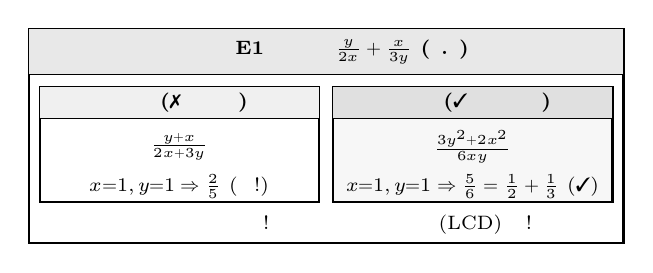
\begin{tikzpicture}[x=1cm, y=1cm, every node/.style={font=\scriptsize, text=black}]
  \draw[black, line width=0.9pt] (0,0) rectangle (7.55,2.72);
  \fill[gray!18] (0,2.14) rectangle (7.55,2.72);
  \draw[black, line width=0.6pt] (0,2.14) -- (7.55,2.14);
  \node at (3.775,2.43) {\textbf{បេសកកម្ម \en{E1}៖ គណនាផលបូក $\tfrac{y}{2x} + \tfrac{x}{3y}$ (ទំ.៨១)}};

  % Student A
  \draw[black, line width=0.7pt] (0.14,0.52) rectangle (3.68,1.98);
  \fill[gray!12] (0.14,1.58) rectangle (3.68,1.98);
  \draw[black, line width=0.45pt] (0.14,1.58) -- (3.68,1.58);
  \node at (1.91,1.78) {\textbf{សិស្ស ក (\ding{55} បូកភាគបែង)}};
  \node at (1.91,1.22) {$\tfrac{y + x}{2x + 3y}$};
  \node at (1.91,0.72) {$x{=}1, y{=}1 \Rightarrow \tfrac{2}{5}$ (ខុស!)};

  % Student B
  \draw[black, line width=0.85pt, fill=gray!6] (3.86,0.52) rectangle (7.41,1.98);
  \fill[gray!24] (3.86,1.58) rectangle (7.41,1.98);
  \draw[black, line width=0.55pt] (3.86,1.58) -- (7.41,1.58);
  \node at (5.635,1.78) {\textbf{សិស្ស ខ (\ding{51} តម្រូវភាគបែង)}};
  \node at (5.635,1.22) {$\tfrac{3y^2 + 2x^2}{6xy}$};
  \node at (5.635,0.72) {$x{=}1, y{=}1 \Rightarrow \tfrac{5}{6} = \tfrac{1}{2}+\tfrac{1}{3}$ (\ding{51})};

  \node at (3.775,0.24) {\textbf{គន្លឹះ៖} ហាមបូកភាគបែងត្រង់ៗ! ត្រូវតម្រូវភាគបែងរួមតូចបំផុត (\en{LCD}) សិន!};
\end{tikzpicture}}

% ២. E2 Explore: ដាក់ភាគបែងជាកត្តា និងតម្រូវភាគបែងរួម (ទំ.៨២ លំហាត់គំរូ ១)
\newcommand{\figExploreRATSixFive}{%
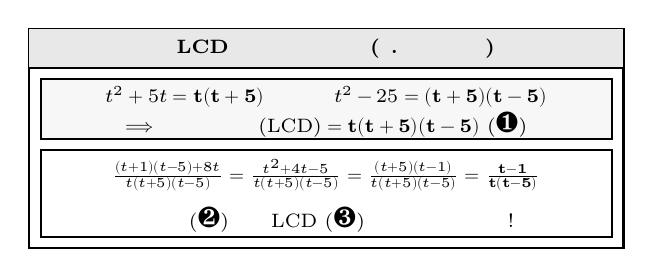
\begin{tikzpicture}[x=1cm, y=1cm, every node/.style={font=\scriptsize, text=black}]
  \draw[black, line width=0.9pt] (0,0) rectangle (7.55,2.78);
  \fill[gray!18] (0,2.28) rectangle (7.55,2.78);
  \draw[black, line width=0.6pt] (0,2.28) -- (7.55,2.28);
  \node at (3.775,2.53) {\textbf{រក \en{LCD} តាមការដាក់ភាគបែងជាកត្តា (ទំ.៨២ លំហាត់គំរូ ១)}};

  \draw[black, line width=0.7pt, fill=gray!6] (0.15,1.38) rectangle (7.40,2.14);
  \node at (3.775,1.92) {$t^2 + 5t = \mathbf{t(t + 5)}$ \quad និង \quad $t^2 - 25 = \mathbf{(t + 5)(t - 5)}$};
  \node at (3.775,1.56) {$\Longrightarrow \text{ភាគបែងរួមតូចបំផុត (\en{LCD})} = \mathbf{t(t + 5)(t - 5)}$ (\cnum{1})};

  \draw[black, line width=0.75pt] (0.15,0.14) rectangle (7.40,1.24);
  \node at (3.775,0.92) {$\tfrac{(t + 1)(t - 5) + 8t}{t(t + 5)(t - 5)} = \tfrac{t^2 + 4t - 5}{t(t + 5)(t - 5)} = \tfrac{(t + 5)(t - 1)}{t(t + 5)(t - 5)} = \mathbf{\tfrac{t - 1}{t(t - 5)}}$};
  \node at (3.775,0.36) {គុណបំពេញ (\cnum{2}) រក្សា \en{LCD} (\cnum{3}) រួចដាក់ភាគយកជាកត្តាសម្រួល!};
\end{tikzpicture}}

% ៣. E3 Explain: ធនាគារហេតុផល ①–④ នៃការបូក-ដកភាគបែងខុសគ្នា (ទំ.៨២)
\newcommand{\figExplainRATSixFive}{%
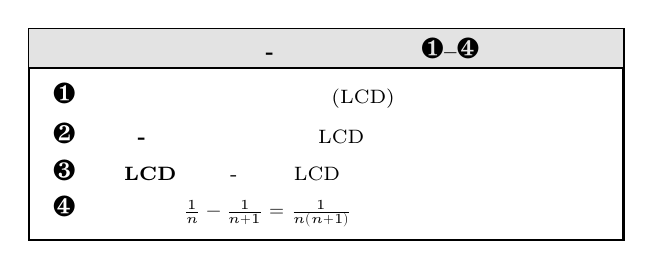
\begin{tikzpicture}[x=1cm, y=1cm, every node/.style={font=\scriptsize, text=black}]
  \draw[black, line width=0.95pt] (0,0) rectangle (7.55,2.68);
  \fill[gray!22] (0,2.18) rectangle (7.55,2.68);
  \draw[black, line width=0.65pt] (0,2.18) -- (7.55,2.18);
  \node at (3.775,2.43) {\textbf{វិធាន ៤ ជំហានបូក-ដកភាគបែងខុសគ្នា និងហេតុផល \cnum{1}--\cnum{4}}};

  \node[anchor=west] at (0.18,1.84) {\cnum{1} \textbf{ដាក់ភាគបែងជាកត្តាសិន៖} កំណត់ភាគបែងរួមតូចបំផុត (\en{LCD})។};
  \node[anchor=west] at (0.18,1.36) {\cnum{2} \textbf{គុណបំពេញលើ-ក្រោម៖} គុណនឹងកត្តាដែលខ្វះក្នុង \en{LCD}។};
  \node[anchor=west] at (0.18,0.88) {\cnum{3} \textbf{ហាមលុប \en{LCD} ចោល៖} បូក-ដកភាគយកលើ \en{LCD} រួចសម្រួលកត្តារួម។};
  \node[anchor=west] at (0.18,0.36) {\cnum{4} \textbf{លំនាំបំបែកតៗគ្នា៖} $\tfrac{1}{n} - \tfrac{1}{n + 1} = \tfrac{1}{n(n + 1)}$ សម្រួលតួកណ្ដាល។};
\end{tikzpicture}}

% ៤. E4 Elaborate: លំហាត់គំរូ ២ (Telescoping Sum ទំ.៨២–៨៣) និងប្រតិបត្តិ គ (ទំ.៨៣)
\newcommand{\figElaborateRATSixFive}{%
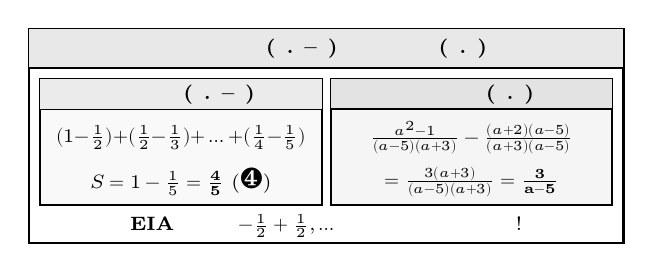
\begin{tikzpicture}[x=1cm, y=1cm, every node/.style={font=\scriptsize, text=black}]
  \draw[black, line width=0.9pt] (0,0) rectangle (7.55,2.72);
  \fill[gray!18] (0,2.22) rectangle (7.55,2.72);
  \draw[black, line width=0.6pt] (0,2.22) -- (7.55,2.22);
  \node at (3.775,2.47) {\textbf{លំនាំសម្រួលតៗគ្នា (ទំ.៨២–៨៣) និងប្រតិបត្តិ គ (ទំ.៨៣)}};

  % Left: Telescoping
  \draw[black, line width=0.75pt, fill=gray!5] (0.14,0.48) rectangle (3.72,2.08);
  \fill[gray!16] (0.14,1.70) rectangle (3.72,2.08);
  \draw[black, line width=0.5pt] (0.14,1.70) -- (3.72,1.70);
  \node at (1.93,1.89) {\textbf{លំហាត់គំរូ ២ (ទំ.៨២–៨៣)}};
  \node at (1.93,1.34) {$(1{-}\tfrac{1}{2}){+}(\tfrac{1}{2}{-}\tfrac{1}{3}){+}\dots{+}(\tfrac{1}{4}{-}\tfrac{1}{5})$};
  \node at (1.93,0.78) {$S = 1 - \tfrac{1}{5} = \mathbf{\tfrac{4}{5}}$ (\cnum{4})};

  % Right: Practice C
  \draw[black, line width=0.8pt, fill=gray!8] (3.84,0.48) rectangle (7.41,2.08);
  \fill[gray!22] (3.84,1.70) rectangle (7.41,2.08);
  \draw[black, line width=0.6pt] (3.84,1.70) -- (7.41,1.70);
  \node at (5.625,1.89) {\textbf{ប្រតិបត្តិ គ (ទំ.៨៣)}};
  \node at (5.625,1.34) {$\tfrac{a^2 - 1}{(a-5)(a+3)} - \tfrac{(a+2)(a-5)}{(a+3)(a-5)}$};
  \node at (5.625,0.78) {$= \tfrac{3(a + 3)}{(a - 5)(a + 3)} = \mathbf{\tfrac{3}{a - 5}}$};

  \node at (3.775,0.22) {\textbf{\en{EIA}៖} តួកណ្ដាល $-\tfrac{1}{2}+\tfrac{1}{2}, \dots$ ស៊ីសងគ្នាអស់ សល់តែតួដើមនិងតួចុង!};
\end{tikzpicture}}

% ៥. E5 Evaluate: ជម្រើសវិនិច្ឆ័យ A-D សម្រាប់រក LCD នៃ 3/(x^2-4) - 1/(x^2+2x)
\newcommand{\figExitRATSixFive}{%
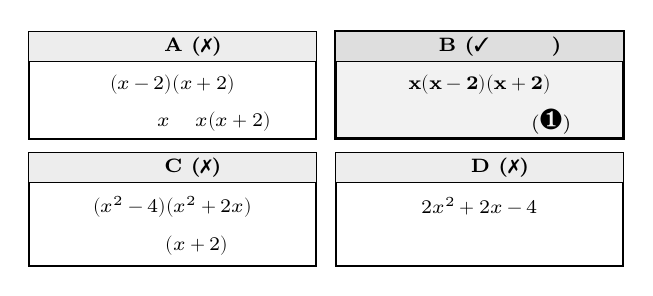
\begin{tikzpicture}[x=1cm, y=1cm, every node/.style={font=\scriptsize, text=black}]
  % Choice A
  \draw[black, line width=0.8pt] (0,1.62) rectangle (3.65,2.98);
  \fill[gray!14] (0,2.60) rectangle (3.65,2.98);
  \draw[black, line width=0.5pt] (0,2.60) -- (3.65,2.60);
  \node at (1.825,2.79) {\textbf{ជម្រើស \en{A} (\ding{55})}};
  \node at (1.825,2.30) {$(x - 2)(x + 2)$};
  \node at (1.825,1.84) {ភ្លេចកត្តាឯកធា $x$ ពី $x(x+2)$};

  % Choice B (Correct)
  \draw[black, line width=1.0pt, fill=gray!10] (3.90,1.62) rectangle (7.55,2.98);
  \fill[gray!26] (3.90,2.60) rectangle (7.55,2.98);
  \draw[black, line width=0.55pt] (3.90,2.60) -- (7.55,2.60);
  \node at (5.725,2.79) {\textbf{ជម្រើស \en{B} (\ding{51} ត្រឹមត្រូវ)}};
  \node at (5.725,2.30) {$\mathbf{x(x - 2)(x + 2)}$};
  \node at (5.725,1.84) {កត្តារួមតូចបំផុតពិតប្រាកដ (\cnum{1})};

  % Choice C
  \draw[black, line width=0.8pt] (0,0) rectangle (3.65,1.44);
  \fill[gray!14] (0,1.06) rectangle (3.65,1.44);
  \draw[black, line width=0.5pt] (0,1.06) -- (3.65,1.06);
  \node at (1.825,1.25) {\textbf{ជម្រើស \en{C} (\ding{55})}};
  \node at (1.825,0.76) {$(x^2 - 4)(x^2 + 2x)$};
  \node at (1.825,0.26) {គុណជាន់កត្តា $(x + 2)$ លើស};

  % Choice D
  \draw[black, line width=0.8pt] (3.90,0) rectangle (7.55,1.44);
  \fill[gray!14] (3.90,1.06) rectangle (7.55,1.44);
  \draw[black, line width=0.5pt] (3.90,1.06) -- (7.55,1.06);
  \node at (5.725,1.25) {\textbf{ជម្រើស \en{D} (\ding{55})}};
  \node at (5.725,0.76) {$2x^2 + 2x - 4$};
  \node at (5.725,0.26) {ច្រឡំយកភាគបែងបូកបញ្ចូលគ្នា};
\end{tikzpicture}}

% ============================================================================
% ៦. ចាប់ផ្ដើមឯកសារ (Document Body)
% ============================================================================
\begin{document}
\fontsize{10pt}{15.2pt}\selectfont

% --- ក្បាលរដ្ឋបាល ៣ ជួរ ---
{\muol
មន្ទីរអប់រំ យុវជន និងកីឡា ខេត្តកំពង់ធំ\\
ការិយាល័យអប់រំ យុវជន និងកីឡា ស្រុកកំពង់ស្វាយ\\
អនុវិទ្យាល័យព្រះក្រសាំង\par}

\vspace{-6pt}
\begin{center}
  \khmflourish\\[2pt]
  {\muol\fontsize{12pt}{18pt}\selectfont កិច្ចតែងការបង្រៀន}
\end{center}
\vspace{2pt}

% --- ព័ត៌មានទូទៅ ---
\begin{tabular}{@{}l@{\hspace{1.8cm}}l@{}}
  \ditem \textbf{មុខវិជ្ជា៖} គណិតវិទ្យា & \ditem \textbf{ថ្នាក់ទី៖} \enbf{8} (ម៉ោងទី៥ នៃមេរៀនទី៦) \\
  \multicolumn{2}{@{}l@{}}{\ditem \textbf{ជំពូកទី២ (ពីជគណិត) -- មេរៀនទី៦៖} កន្សោមសនិទាន (សៀវភៅសិក្សាគោល ទំព័រ \en{75--88})} \\
  \multicolumn{2}{@{}l@{}}{\ditem \textbf{ខ្លឹមសារបង្រៀន៖} \textbf{៥.២ វិធីបូកនិងវិធីដកកន្សោមសនិទានមានភាគបែងមិនដូចគ្នា} (ទំព័រ \en{81--83, 86, 88})} \\
  \ditem \textbf{រយៈពេល៖} \en{50} នាទី (\en{1} ម៉ោងសិក្សា) & \ditem \textbf{កាលបរិច្ឆេទ៖} ថ្ងៃសុក្រ ទី១៨ ខែធ្នូ ឆ្នាំ២០២៦
\end{tabular}

\vspace{5pt}

% --- I. វត្ថុបំណង ---
{\muol \enbf{I.} វត្ថុបំណង}\par
\vspace{2pt}
ក្រោយពីបញ្ចប់មេរៀននេះ សិស្សមានសមត្ថភាព៖
\begin{itemize}[leftmargin=1.35cm, label=\wcirc, itemsep=1pt, topsep=2pt, parsep=0pt]
  \item \textbf{វិជ្ជាសម្បទា៖} ប្រាប់វិធានទាំង ៤ ជំហាននៃការបូក និងការដកកន្សោមសនិទានដែលមានភាគបែងមិនដូចគ្នា (ដាក់ភាគបែងជាកត្តា រកភាគបែងរួមតូចបំផុត \en{LCD} គុណបំពេញលើ-ក្រោម និងបូក-ដកភាគយកលើភាគបែងរួម) បានត្រឹមត្រូវតាមសៀវភៅសិក្សាគោល (ទំព័រ ៨១–៨២)។
  \item \textbf{បំណិនសម្បទា៖} គណនាផលបូក និងផលដកកន្សោមសនិទានដែលមានភាគបែងមិនដូចគ្នា ព្រមទាំងអនុវត្តលំនាំបំបែក $\dfrac{1}{n} - \dfrac{1}{n+1} = \dfrac{1}{n(n+1)}$ ដើម្បីគណនាផលបូកប្រភាគតៗគ្នាក្នុងសន្លឹកកិច្ចការបំពេញចន្លោះបានត្រឹមត្រូវ។
  \item \textbf{ចរិយាសម្បទា៖} មានទម្លាប់ដាក់ភាគបែងជាកត្តាសិនមុនរកភាគបែងរួម មិនច្រឡំបូកភាគបែងត្រង់ៗ និងមិនលុបភាគបែងរួមចោលក្នុងពេលសម្រួលកន្សោមសនិទាន។
\end{itemize}

\vspace{4pt}

% --- II. សម្ភារៈឧបទេស (Zero-LCD & Fill-In Worksheet Mode) ---
{\muol \enbf{II.} សម្ភារៈឧបទេស}\par
\vspace{2pt}
\begin{itemize}[leftmargin=1.35cm, label=\wcirc, itemsep=1pt, topsep=2pt, parsep=0pt]
  \item \textbf{សម្រាប់គ្រូ៖} សៀវភៅសិក្សាគោលគណិតវិទ្យាថ្នាក់ទី៨ (ទំព័រ ៨១–៨៣, ៨៦, ៨៨) ក្ដារខៀន ដីសស និងប្លង់ក្ដារខៀន ៣ ផ្នែក (គ្មានស្លាយ \en{LCD} និងគ្មានឧបករណ៍កាត់បិទ)។
  \item \textbf{សម្រាប់សិស្ស៖} \textbf{សន្លឹកកិច្ចការសិស្សបំពេញចន្លោះ ស-ខ្មៅ} (បោះពុម្ពសងខាង ១ សន្លឹកក្នុងម្នាក់ សម្រាប់បំពេញតាមជំហាន \en{E1--E5}) សៀវភៅសិក្សាគោល និងប៊ិច។
\end{itemize}

\vspace{4pt}

% --- III. វិធីសាស្រ្តបង្រៀន ---
{\muol \enbf{III.} វិធីសាស្រ្តបង្រៀន}\par
\vspace{2pt}
\begin{itemize}[leftmargin=1.35cm, label=\wcirc, itemsep=1pt, topsep=2pt, parsep=0pt]
  \item គោលវិធីសិស្សមជ្ឈមណ្ឌល តាមលំនាំរិះរក \textbf{\en{5Es} (\en{Engage, Explore, Explain, Elaborate, Evaluate})} ដោយប្រើសន្លឹកកិច្ចការបំពេញចន្លោះជាគោល។
  \item យុទ្ធសាស្ត្រផ្អែកលើការស្រាវជ្រាវគរុកោសល្យអន្តរជាតិ៖ \textbf{ការវិភាគកំហុសបូកភាគបែង និងការរក្សាភាគបែងរួម \en{LCD}} (\en{Lee \& Boyadzhiev, 2020; Siegler \& Lortie-Forgues, 2015}) និង \textbf{លំនាំបំបែកប្រភាគសម្រួលតៗគ្នា} (\en{Rittle-Johnson \& Star, 2007})។
\end{itemize}

\vspace{4pt}

% --- IV. ដំណើរការបង្រៀន (50 នាទី) ---
{\muol \enbf{IV.} ដំណើរការបង្រៀន}\par
\vspace{2pt}

\renewcommand{\arraystretch}{1.15}
\begin{longtable}{|L{5.50cm}|L{7.90cm}|L{4.80cm}|}
\hline
\multicolumn{1}{|c|}{\cellcolor{headgray}\textbf{សកម្មភាពគ្រូ}} &
\multicolumn{1}{c|}{\cellcolor{headgray}\textbf{ខ្លឹមសារមេរៀន}} &
\multicolumn{1}{c|}{\cellcolor{headgray}\textbf{សកម្មភាពសិស្ស}} \\
\hline
\endfirsthead

\hline
\multicolumn{1}{|c|}{\cellcolor{headgray}\textbf{សកម្មភាពគ្រូ}} &
\multicolumn{1}{c|}{\cellcolor{headgray}\textbf{ខ្លឹមសារមេរៀន}} &
\multicolumn{1}{c|}{\cellcolor{headgray}\textbf{សកម្មភាពសិស្ស}} \\
\hline
\endhead

\hline
\endfoot

% ==================== ជំហានទី១ (2min) ====================
\stepheader{ជំហានទី១ \enbf{(}រដ្ឋបាលថ្នាក់\enbf{)} \timenote{(2min)}}
$\bullet$ ពិនិត្យអនាម័យ សណ្ដាប់ធ្នាប់ និងវត្តមានសិស្ស \par
$\bullet$ ចែក \textbf{សន្លឹកកិច្ចការបំពេញចន្លោះ} ដល់សិស្សគ្រប់គ្នា
&
$\bullet$ វត្តមានសិស្ស៖ \dotfill នាក់ (អវត្តមាន៖ \dotfill នាក់) \par
$\bullet$ ត្រៀមសៀវភៅគោល (ទំ.៨១–៨៣) និងសន្លឹកកិច្ចការសិស្ស
&
$\circ$ ប្រធានថ្នាក់រាយការណ៍វត្តមាន \par
$\circ$ ទទួលសន្លឹកកិច្ចការ និងសរសេរឈ្មោះ \\
\hline

% ==================== ជំហានទី២ (9min) ====================
\stepheader{ជំហានទី២ \enbf{(}ពិនិត្យកិច្ចការចាស់ \enbf{+} រំលឹកមេរៀន \enbf{+} \enbf{E1}\enbf{)} \timenote{(9min)}}
\redsub{$\bullet$ ពិនិត្យកិច្ចការផ្ទះ} \timenote{(កុំឱ្យលើស 3min)} \par
$\bullet$ ហៅសិស្ស ២ នាក់ឡើងសរសេរចម្លើយកិច្ចការផ្ទះម៉ោងមុន (ទំ.៨៦ \en{\#7} ខ, ឃ, ច, ឈ) លើក្ដារខៀនផ្នែកខាងឆ្វេង
&
\textbf{កំណែកិច្ចការផ្ទះ (ទំ.៨៦ លេខ ៧ ខ, ឃ, ច, ឈ)៖} \par
$\bullet$ ខ) $\dfrac{y}{14} - \dfrac{3y}{14} = -\dfrac{2y}{14} = -\dfrac{y}{7}$ \quad ; \quad ឃ) $\dfrac{y}{b+6} + \dfrac{2y}{b+6} = \dfrac{3y}{b+6}$ \par
$\bullet$ ច) $\dfrac{a+b}{x-3} - \dfrac{a+b}{3-x} = \dfrac{2(a+b)}{x-3}$ \quad ; \quad ឈ) $\dfrac{x^2 + 2x + 1}{x^2 - 1} = \dfrac{x + 1}{x - 1}$
&
$\circ$ សិស្ស ២ នាក់ឡើងសរសេរចម្លើយ \par
$\circ$ ផ្ទៀងផ្ទាត់ និងកែចម្លើយក្នុងសៀវភៅ \\[3pt]

\redsub{$\bullet$ រំលឹកមេរៀនចាស់} \timenote{(3min)} \par
$\bullet$ សួរផ្ទាល់មាត់រំលឹកការបូកប្រភាគលេខមានភាគបែងខុសគ្នា និងការរកពហុគុណរួមតូចបំផុត \par
\hspace*{0.3em}– សំណួរ៖ «តើ $\dfrac{1}{2} + \dfrac{1}{3}$ ស្មើប៉ុន្មាន? ហើយពហុគុណរួមតូចបំផុតនៃ $2x$ និង $3y$ គឺអ្វី?»
&
\textbf{រំលឹកការបូកប្រភាគភាគបែងខុសគ្នា៖} \par
$\bullet$ ប្រភាគលេខ៖ $\dfrac{1}{2} + \dfrac{1}{3} = \dfrac{1 \cdot 3}{6} + \dfrac{1 \cdot 2}{6} = \dfrac{5}{6}$ (\textbf{មិនមែន} $\dfrac{1+1}{2+3} = \dfrac{2}{5}$ ទេ!)។ \par
$\bullet$ ភាគបែងរួមតូចបំផុតនៃ $2x$ និង $3y$ គឺ $\mathbf{6xy}$ ។
&
$\circ$ ឆ្លើយផ្ទាល់មាត់៖ $\dfrac{1}{2} + \dfrac{1}{3} = \dfrac{5}{6}$ ហើយភាគបែងរួមនៃ $2x$ និង $3y$ គឺ $6xy$ \\[3pt]

\fiveE{E1 - Engage} \timenote{(3min)} \par
$\bullet$ សរសេរឧទាហរណ៍ទំ.៨១ $\dfrac{y}{2x} + \dfrac{x}{3y}$ លើក្ដារខៀន ហើយឱ្យសិស្សវិនិច្ឆ័យចម្លើយ \textbf{សិស្ស ក} និង \textbf{សិស្ស ខ} ក្នុងប្រអប់ \en{E1}
&
\textbf{៥.២ ករណីមានភាគបែងមិនដូចគ្នា (ទំ.៨១)} \par
$\bullet$ \textbf{បេសកកម្ម \en{E1}៖} គណនាផលបូក $\dfrac{y}{2x} + \dfrac{x}{3y}$ (ទំ.៨១)៖ \par
\hspace*{0.4em}– \textbf{សិស្ស ក} ឆ្លើយ $\dfrac{y + x}{2x + 3y}$ \quad ឯ \textbf{សិស្ស ខ} ឆ្លើយ $\dfrac{3y^2 + 2x^2}{6xy}$ ។
&
$\circ$ គូសធីកជ្រើសរើសចម្លើយ និងសាកជំនួសលេខ $x = 1, y = 1$ ក្នុងប្រអប់ \en{E1} \\[3pt]

$\bullet$ ឱ្យសិស្សសាកជំនួស $x = 1, y = 1$ ដើម្បីរកអ្នកត្រូវ រួចភ្ជាប់ចូលចំណងជើងមេរៀនថ្ងៃនេះ
&
\cfig{\figEngageRATSixFive}
&
$\circ$ រកឃើញថាសិស្ស ក ខុស ($\frac{2}{5} \neq \frac{5}{6}$) ព្រោះច្រឡំបូកភាគបែងត្រង់ៗ! \\
\hline

% ==================== ជំហានទី៣ (17min) ====================
\stepheader{ជំហានទី៣ \enbf{(}មេរៀនថ្មី៖ \enbf{E2 + E3}\enbf{)} \timenote{(17min)}}
\fiveE{E2 - Explore} \timenote{(11min)} \par
$\bullet$ \textbf{ផ្នែក \en{E2-A} (៥ នាទី)៖} ឱ្យសិស្សធ្វើការជាដៃគូបំពេញចន្លោះឧទាហរណ៍ ក និង ខ (ទំ.៨១–៨២) លើសន្លឹកកិច្ចការទំព័រ ១
&
\textbf{សកម្មភាពរុករកទី១ (\en{E2-A})៖ ភាគបែងឯកធា និងទ្វេធា (ទំ.៨១–៨២)} \par
$\bullet$ \textbf{ក)} $\dfrac{y}{2x} + \dfrac{x}{3y}$ (ភាគបែងរួម $\text{\en{LCD}} = 6xy$)៖ \par
\hspace*{0.4em}$\dfrac{y \cdot 3y}{2x \cdot 3y} + \dfrac{x \cdot 2x}{3y \cdot 2x} = \dfrac{3y^2}{6xy} + \dfrac{2x^2}{6xy} = \mathbf{\dfrac{3y^2 + 2x^2}{6xy}}$ ។
&
$\circ$ ពិភាក្សាជាដៃគូ កំណត់កត្តាខ្វះ $3y$ និង $2x$ រួចបំពេញចន្លោះឧទាហរណ៍ ក \\[3pt]

$\bullet$ ដើរពិនិត្យការគុណពន្លាតដក $-2n$ ក្នុងឧទាហរណ៍ ខ ដើម្បីកុំឱ្យសិស្សភ្លេចវង់ក្រចក
&
$\bullet$ \textbf{ខ)} $\dfrac{4}{n} - \dfrac{2}{n + 1}$ ($\text{\en{LCD}} = n(n + 1)$)៖ \par
\hspace*{0.4em}$\dfrac{4(n + 1) - 2n}{n(n + 1)} = \dfrac{4n + 4 - 2n}{n(n + 1)} = \dfrac{2n + 4}{n(n + 1)} = \mathbf{\dfrac{2(n + 2)}{n(n + 1)}}$ ។
&
$\circ$ គណនាផលដក ខ រួចទាញកត្តារួម $2$ ពីភាគយក $2n + 4 = 2(n + 2)$ \\[3pt]

$\bullet$ \textbf{ផ្នែក \en{E2-B} (៦ នាទី)៖} ណែនាំលំហាត់គំរូទី ១ (ទំ.៨២) ដែលភាគបែងជាពហុធាត្រូវដាក់ជាកត្តាសិនមុនរក \en{LCD} \par
\hspace*{0.3em}– សំណួរ៖ «តើ $t^2 + 5t$ និង $t^2 - 25$ មានកត្តារួមអ្វីដូចគ្នា?»
&
\textbf{សកម្មភាពរុករកទី២ (\en{E2-B})៖ ភាគបែងពហុធា (លំហាត់គំរូ ១ ទំ.៨២)} \par
$\bullet$ គណនា $\dfrac{t + 1}{t^2 + 5t} + \dfrac{8}{t^2 - 25}$៖ \par
\hspace*{0.4em}– ដាក់ភាគបែងជាកត្តា៖ $t^2 + 5t = t(t + 5)$ ; $t^2 - 25 = (t + 5)(t - 5)$ \par
\hspace*{0.4em}– ភាគបែងរួមតូចបំផុត៖ $\text{\en{LCD}} = \mathbf{t(t + 5)(t - 5)}$ ។
&
$\circ$ ដាក់ភាគបែងទាំងពីរជាកត្តា រកឃើញកត្តារួម $(t + 5)$ នាំឱ្យ $\text{\en{LCD}} = t(t+5)(t-5)$ \\[3pt]

$\bullet$ គូសតារាងដំណោះស្រាយលើក្ដារខៀន ឱ្យសិស្សផ្ទៀងផ្ទាត់ការសម្រួលកត្តា $(t + 5)$ ចុងក្រោយ
&
\cfig{\figExploreRATSixFive}
&
$\circ$ បំពេញការពន្លាត $(t+1)(t-5) + 8t = t^2 + 4t - 5 = (t+5)(t-1)$ រួចសម្រួល $(t+5)$ \\[3pt]

\fiveE{E3 - Explain} \timenote{(6min)} \par
$\bullet$ ឱ្យតំណាងដៃគូ ២ ក្រុមឡើងបង្ហាញចម្លើយ \en{E2-A} និង \en{E2-B} រួចទាញវិធាន ៤ ជំហាន (ទំ.៨២)
&
\textbf{វិធានបូក-ដកកន្សោមសនិទានភាគបែងខុសគ្នា (ទំ.៨២)៖} \par
$\bullet$ \textbf{១)} ដាក់ភាគបែងនីមួយៗជាផលគុណកត្តាដើម្បីរកភាគបែងរួមតូចបំផុត (\en{LCD})។ \par
$\bullet$ \textbf{២)} គុណបំពេញភាគយកនិងភាគបែងនីមួយៗឱ្យមានភាគបែងដូចគ្នា រួចបូកឬដកភាគយកលើ \en{LCD} ហើយសម្រួលលទ្ធផល (បើអាច)។
&
$\circ$ តំណាងក្រុមឡើងបកស្រាយ \par
$\circ$ សិស្សទាំងអស់បំពេញប្រអប់វិធាន \en{E3} លើសន្លឹកកិច្ចការទំព័រ ២ \\[3pt]

$\bullet$ សង្ខេប \textbf{ធនាគារហេតុផល \cnum{1}--\cnum{4}} លើក្ដារខៀនកណ្ដាលទុកជាគោលការណ៍យោង
&
\cfig{\figExplainRATSixFive}
&
$\circ$ កត់ចំណាំលេខកូដហេតុផល \cnum{1}--\cnum{4} ទុកការពារកំហុសលុប \en{LCD} ចោល \\
\hline

% ==================== ជំហានទី៤ (20min) ====================
\stepheader{ជំហានទី៤ \enbf{(}ពង្រឹងពុទ្ធិ និងវាយតម្លៃ៖ \enbf{E4 + E5}\enbf{)} \timenote{(20min)}}
\fiveE{E4 - Elaborate} \timenote{(10min)} \par
$\bullet$ ណែនាំលំហាត់គំរូទី ២ (ទំ.៨២–៨៣) និងប្រតិបត្តិ គ (ទំ.៨៣) ក្នុងប្រអប់ \en{E4} លើសន្លឹកកិច្ចការទំព័រ ២ \par
$\bullet$ ឱ្យសិស្សស្រាយបញ្ជាក់ $\dfrac{1}{n} - \dfrac{1}{n+1} = \dfrac{1}{n(n+1)}$ ជាមុនសិន
&
\textbf{ការពង្រីកចំណេះដឹង (\en{E4})៖ លំហាត់គំរូ ២ និងប្រតិបត្តិ គ (ទំ.៨២–៨៣)} \par
$\bullet$ \textbf{១) លំហាត់គំរូ ២ (ទំ.៨២–៨៣)៖} \par
\hspace*{0.4em}– ក) $\dfrac{1}{n} - \dfrac{1}{n + 1} = \dfrac{(n + 1) - n}{n(n + 1)} = \mathbf{\dfrac{1}{n(n + 1)}}$ (\cnum{4}) \par
\hspace*{0.4em}– ខ) គណនា $S = \dfrac{1}{1 \cdot 2} + \dfrac{1}{2 \cdot 3} + \dfrac{1}{3 \cdot 4} + \dfrac{1}{4 \cdot 5} = 1 - \dfrac{1}{5} = \mathbf{\dfrac{4}{5}}$ ។
&
$\circ$ គណនាផលដក $\dfrac{1}{n} - \dfrac{1}{n+1}$ រួចយកលំនាំនេះបំបែកផលបូក $S$ ជា ៤ គូ \\[3pt]

$\bullet$ ឱ្យសិស្សគណនាប្រតិបត្តិ គ (ទំ.៨៣) ដោយដាក់ $a^2 - 2a - 15 = (a - 5)(a + 3)$ ជាកត្តា
&
$\bullet$ \textbf{២) ប្រតិបត្តិ គ (ទំ.៨៣)៖} $\dfrac{a^2 - 1}{a^2 - 2a - 15} - \dfrac{a + 2}{a + 3}$ \par
\hspace*{0.4em}$= \dfrac{(a^2 - 1) - (a + 2)(a - 5)}{(a - 5)(a + 3)} = \dfrac{3a + 9}{(a - 5)(a + 3)} = \dfrac{3(a + 3)}{(a - 5)(a + 3)} = \mathbf{\dfrac{3}{a - 5}}$ ។
&
$\circ$ ពន្លាត $-(a^2 - 3a - 10) = -a^2 + 3a + 10$ ដោយប្រុងប្រយ័ត្នសញ្ញាដក \\[3pt]

$\bullet$ សួរសំណួរ \textbf{\en{EIA Looking-Back}}៖ «តើលំនាំបំបែក $\dfrac{1}{n(n+1)}$ លឿនជាងការតម្រូវភាគបែងលេខ $2, 6, 12, 20$ យ៉ាងដូចម្ដេច?»
&
\cfig{\figElaborateRATSixFive}
&
$\circ$ ឆ្លើយសំណួរ \en{EIA}៖ ព្រោះតួកណ្ដាលស៊ីសងគ្នាសូន្យអស់ ទោះបូកដល់ $\frac{1}{99\cdot 100}$ ក៏គិតបានភ្លាម! \\[3pt]

\fiveE{E5 - Evaluate} \timenote{(10min)} \par
$\bullet$ \textbf{ហ្វឹកហាត់ក្រុមតូច (៥ នាទី)៖} ឱ្យសិស្សធ្វើលំហាត់ទំ.៨៦ \en{\#8} (ក, គ, ង) និងទំ.៨៨ \en{\#14} (ខ) ក្នុងសន្លឹកកិច្ចការ \par
\hspace*{0.3em}– \textbf{ផ្អាកសួរ (\en{Pause-Review})៖} ផ្ទៀងផ្ទាត់ការទាញកត្តា $2a + 6 = 2(a + 3)$ ក្នុង \en{\#8} ង
&
\textbf{ហ្វឹកហាត់លំហាត់សៀវភៅគោល (ទំ.៨៦ \en{\#8} និង ទំ.៨៨ \en{\#14})៖} \par
$\bullet$ \en{\#8} ក) $\dfrac{5x}{2} - \dfrac{2x + 3y}{4} = \dfrac{10x - (2x + 3y)}{4} = \mathbf{\dfrac{8x - 3y}{4}}$ \par
$\bullet$ \en{\#8} គ) $\dfrac{5}{xy} + \dfrac{6}{yz} = \mathbf{\dfrac{5z + 6x}{xyz}}$ \quad ; \quad ង) $\dfrac{4a}{2(a + 3)} + \dfrac{3}{a + 3} = \mathbf{\dfrac{2a + 3}{a + 3}}$ \par
$\bullet$ \en{\#14} ខ) $\dfrac{1}{50} - \dfrac{1}{51} = \dfrac{1}{50 \times 51} = \mathbf{\dfrac{1}{2550}}$ (\cnum{4})
&
$\circ$ គណនាបំពេញចន្លោះជាក្រុម ៤ នាក់ និងផ្ទៀងផ្ទាត់ហេតុផល \cnum{1}--\cnum{4} ជាមួយមិត្តរួមតុ \\[3pt]

$\bullet$ \textbf{បិទបញ្ចប់បេសកកម្ម \en{E1} + ល្បឿនវិនិច្ឆ័យ \en{A--D} (៣ នាទី)៖} សួររក \en{LCD} នៃកន្សោម $\dfrac{3}{x^2 - 4} - \dfrac{1}{x^2 + 2x}$
&
\textbf{សំណួរវិនិច្ឆ័យរហ័ស (\en{60} វិនាទី)៖} តើភាគបែងរួមតូចបំផុត (\en{LCD}) នៃ $\dfrac{3}{x^2 - 4} - \dfrac{1}{x^2 + 2x}$ គឺជម្រើសណា? (\textbf{ចម្លើយត្រូវ៖ \en{B}})
&
$\circ$ បញ្ជាក់ថាសិស្ស ខ ក្នុង \en{E1} ត្រឹមត្រូវ \par
$\circ$ គូសរង្វង់ជម្រើស \en{B} និងប្រាប់មូលហេតុ \\[3pt]

$\bullet$ បង្ហាញការវិភាគជម្រើសទាំង ៤ លើក្ដារខៀន រួចឱ្យសិស្សធ្វើ \textbf{ប័ណ្ណចាកចេញបុគ្គល} (\en{2} នាទីចុងក្រោយ)
&
\cfig{\figExitRATSixFive}
&
$\circ$ ផ្ទៀងផ្ទាត់កំហុសក្នុងជម្រើស \en{A, C, D} \\[3pt]

$\bullet$ ឱ្យសិស្សម្នាក់ៗធ្វើប្រអប់ \textbf{ប័ណ្ណចាកចេញ} (ទំ.៨៦ \en{\#8} ឃ) ដោយខ្លួនឯងមុនប្រមូលសន្លឹកកិច្ចការ
&
\textbf{ប័ណ្ណចាកចេញបុគ្គល (ទំ.៨៦ \en{\#8} ឃ)៖} \par
$\bullet$ គណនា៖ $\dfrac{3c}{2ab} - \dfrac{a}{4bc} = \dfrac{3c \cdot 2c - a \cdot a}{4abc} = \mathbf{\dfrac{6c^2 - a^2}{4abc}}$ ។
&
$\circ$ គណនាប័ណ្ណចាកចេញបុគ្គលលើសន្លឹកកិច្ចការទំព័រ ២ រួចប្រគល់ជូនគ្រូ \\
\hline

% ==================== ជំហានទី៥ (≤2min) ====================
\stepheader{ជំហានទី៥ \enbf{(}កិច្ចការផ្ទះ \enbf{+} បណ្ដាំផ្ញើ\enbf{)}}
\timenote{ចំណាយពេលឱ្យតិចបំផុតកុំឱ្យលើស 2min} \par
$\bullet$ ណែនាំប្រអប់កិច្ចការផ្ទះលើសន្លឹកកិច្ចការទំព័រ ២ (ទំ.៨៦ \en{\#8} និង ទំ.៨៨ \en{\#14})
&
\centering\textbf{កិច្ចការផ្ទះ (សៀវភៅគោល ទំ.៨៦ លេខ ៨ និង ទំ.៨៨ លេខ ១៤)}\par\raggedright
$\bullet$ \textbf{១) ទំ.៨៦ \en{\#8} ខ, ឆ, ឈ៖} គណនា $\dfrac{2x+y}{3} - \dfrac{x-5y}{6}$ , $\dfrac{b^2}{b^2-4b} - \dfrac{b}{b-4}$ និង $\dfrac{a+2}{2a-8} + \dfrac{a-1}{3a-12}$ ។ \par
$\bullet$ \textbf{២) ទំ.៨៨ \en{\#14} ក, គ៖} បង្ហាញថា $\dfrac{1}{8\times 9} = \dfrac{1}{8} - \dfrac{1}{9}$ និងរកចំនួនគត់ $a, b$ ដើម្បីឱ្យ $\dfrac{1}{a} - \dfrac{1}{b} = \dfrac{1}{18\times 19}$ ។
&
$\circ$ គូសចំណាំកិច្ចការផ្ទះលើសន្លឹកកិច្ចការ \\[3pt]

$\bullet$ ផ្តាំផ្ញើឱ្យអានមុនចំណុចទី \textbf{៦. កន្សោមសនិទានដែលមានទម្រង់ប្រភាគលើប្រភាគ} (ទំ.៨៣–៨៤)
&
$\bullet$ \textbf{បណ្ដាំផ្ញើ៖} ធ្វើកិច្ចការផ្ទះឱ្យបានគ្រប់គ្នា និងអានមុនចំណុចទី ៦ (ប្រភាគលើប្រភាគ ទំ.៨៣–៨៤) ។
&
$\circ$ កត់ត្រាបណ្ដាំផ្ញើ ទុកសន្លឹកកិច្ចការក្នុងសៀវភៅ និងជម្រាបលាគ្រូ \\
\hline
\end{longtable}

\vspace{6pt}

% --- ហត្ថលេខា (Signature Block) ---
\begin{flushright}
  \begin{minipage}{9.5cm}
    \centering
    ថ្ងៃសុក្រ ៩កើត ខែមិគសិរ ឆ្នាំមមី អដ្ឋស័ក ពុទ្ធសករាជ ២៥៧០\\
    កំពង់ស្វាយ, ថ្ងៃទី១៨ ខែធ្នូ ឆ្នាំ២០២៦\\[4pt]
    {\muol គ្រូបង្រៀន}\\[32pt]
    \hfill{\muol ហុក ប៊ុនថែន}\hspace*{1.4cm}
  \end{minipage}
\end{flushright}

\end{document}
